\maketitle
\setcounter{page}{1}
\tableofcontents
\newpage
\pagenumbering{arabic}
\section{Theorie}
Atomkerne zerfallen, wenn das Verhältnis zwischen Anzahl von Neutronen und Protonen
bestimmte Grenzen überschreitet. Eine wichtige Größe zum Zerfall von Atomen in die
Halbwertszeit $T$. Diese bezeichnet den Zeitraum, in dem die Hälfte der instabilen Kerne
zerfallen ist. In diesem Versuch wird eine Methode diskutiert, die Halbwertszeit von Nukliden zu bestimmen,
deren $T$ in der Größenordnung Sekunden bis Stunden liegt. Da diese zu Beginn der Messung hergestellt
werden müssen, geschieht dies durch den Beschuss stabiler Kerne mit Neutronen, da diese die Coulomb-Barriere
nicht überwinden müssen. Im folgenden wird diese Kernreaktion betrachtet.

Sobald ein Neutron von einem Kern A aufgenommen wurde,  entsteht ein neuer Kern A*, den man Compound -
oder Zwischenkern nennt. Ihn unterscheidet von seinem Vorgänger die kinetische und Bindungsenergie
des Neutrons. Diese Energie verteilt sich auf viele Nukleonen, die dadurch in höhere Energiezustände
gebracht werden. Deswegen ist es nicht möglich, dass der Kern das neue Nukleon oder ein anderes abstößt.
Aus diesem Grund geht der Kern nach der Emmission eines $\gamma$ - Quants wieder in seinen Grundzustand über:
\begin{equation*}
    \ce{^{m}_{z}A} + \ce{^{1}_{0} n} \rightarrow \ce{^{m + 1}_{z}A^*} \rightarrow \ce{^{m + 1}_{z}A} + \gamma
\end{equation*}
mit m als Massenzahl und z als Kernladungszahl. Der neue Kern $\ce{^{m + 1}_{z}A}$ ist nicht mehr stabil,
da er mehr Neutronen als ein stabiler Kern enthält. Er zerfällt nach längerer Zeit nach folgender Gleichung:
\begin{equation*}
    \ce{^{m + 1}_{z}A} \rightarrow \ce{^{m+1}_{z+1}C} + \symup{\beta}^- + \symup{E_{kin}} + \overline{\symup{\nu}}_{\symup{e}}
\end{equation*}
mit $\overline{\symup{\nu}}_{\symup{e}}$ als Antineutrino. Der Massendefekt in der obigen Gleichung wird
durch die kinetische Energie von Elektron und Antineutrino ausgeglichen.

Der Wirkungsquerschnitt $\sigma$ gibt die Wahrscheinlichkeit an, mit der ein Neutron von einem stabilen Kern
absorbiert wird. Er ist definiert durch
\begin{equation}
  \sigma = \frac{u}{nKd}
  \label{eqn:1}
\end{equation}
mit $u$ als Anzahl der Treffer, $n$ als Anzahl Neutronen pro Sekunde und $d$ als Dicke und $K$ als Atome pro $\symup{cm}^3$
einer \SI{1}{\centi\meter\squared} breiten Folie. Der Wirkungsquerschnitt ist stark geschwindigkeitsanhängig.
Wenn die Geschwindigkeit des Neutrons hoch genug ist, dass die De-Broglie Wellenlänge klein gegen den Radius
des Kerns ist, kann geometrische Optik angewendet werden und es müssen keine Interferenzeffekte betrachtet werden.
Damit Resonanzabsorption auftritt muss die Energie des Neutrons der Differenz zweier Energieniveaus von A* entsprechen.
Aus einer Formel von Breit und Wigner folgt somit die Relation
\begin{equation*}
  \sigma \propto \frac{1}{v} \, .
\end{equation*}
Daraus wird bestätigt, dass bei kleinen Geschwindigkeiten die Wahrscheinlichkeit steigt, dass
das Neutron vom Kern aufgenommen wird.\\
\\
Da Neutronen instabil ist als freies Teilchen, müssen sie vor dem Versuch erzeugt werden. Dabei läuft
folgende Reaktion ab:
\begin{equation*}
  \ce{^{9}_{4}Be} + \ce{^{4}_{2}He} \rightarrow \ce{^{12}_{6}C} + \ce{^{1}_{0}\symup{n}}
\end{equation*}
Die $\alpha$-Teilchen stammen aus dem Zerfall von $\ce{^{226}Ra}$. Die Neutronen werden nun noch abgebremst,
da aufgrund obiger Überlegungen niederenergetische Neutronen am besten geeignet sind. Zu diesem Zweck
werden die Neutronen auf dicke Materieschichten mit leichten Atomkernen geschossen, damit sie wegen
elastischen Stößen Energie abgeben. Aus dem Gesetz zum elatischen Stoß folgt, dass die Energieübertragung
maximiert wird, falls die Massen der Stoßpartner gleich sind. Dafür bietet sich Wasserstoff an.
Der Aufbau zur Erzeugung der niederenergetischen Elektronen ist in Abbildung \ref{fig:2} abgebildet.
\begin{figure}
  \centering
  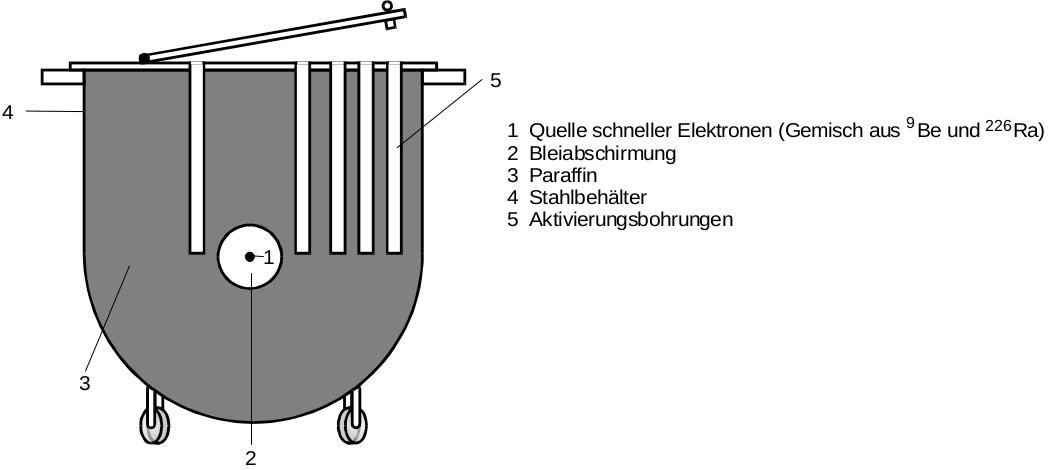
\includegraphics[scale=0.4]{quelle.png}
  \caption{Quelle zur Erzeugung von niederenergetischen Neutronen \cite{anleitung}.}
  \label{fig:2}
\end{figure}
Die Neutronen, die diese Apparatur verlassen, haben eine Energie von \SI{0.025}{\electronvolt} bei einer
Temperatur von \SI{290}{\kelvin}. Daraus folgt eine mittlere Neutronengeschwindigkeit von \SI{2.2}{\kilo\meter\per\second}.
Solche Neutronen werden als thermische Neutronen bezeichnet. \\
\\
In diesem Versuch werden folgende Zerfälle untersucht:
\begin{align}
  \ce{^{115}_{49}In} \, +& \, \symup n \rightarrow   \ce{^{116}_{49}In} \rightarrow  \ce{^{116}_{50}Sn} + \symup{\beta}^- + \overline{\symup{\nu}}_{\symup{e}} \\
  \ce{^{107}_{47}Ag} \, +& \, \symup n \rightarrow   \ce{^{108}_{47}Ag} \rightarrow  \ce{^{108}_{50}Cd} + \symup{\beta}^- + \overline{\symup{\nu}}_{\symup{e}} \label{eqn:2}\\
  \ce{^{109}_{47}Ag} \, +& \, \symup n \rightarrow   \ce{^{110}_{47}Ag} \rightarrow  \ce{^{110}_{48}Cd} + \symup{\beta}^- + \overline{\symup{\nu}}_{\symup{e}} \label{eqn:3}
\end{align}
Dabei ist jedoch für Silber eine Besonderheit zu beachten: Silber liegt in der Natur zu 52,3 \% als $\ce{^{107}Ag}$
und zu 48,7 \% als $\ce{^{109}Ag}$. Die Zerfälle \eqref{eqn:2} und \eqref{eqn:3} laufen gleichzeitig ab und
die Gesamtaktivität besteht aus der Addition der beiden Einzelaktivitäten. Da $\ce{^{110}Ag}$ aber sehr kurzlebig
ist, kommt nach einiger Zeit $t^*$ sämtliche Aktivität nur noch von $\ce{^{108}Ag}$ (siehe Abbildung \ref{fig:3}). Über diese Relation und das
Zerfallsgesetz
\begin{equation}
  N(t) = N_0 \, e^{-\lambda t}
  \label{eqn:4}
\end{equation} mit $\lambda$ als Zerfallskonstante und $N_0 = N(0)$ lassen sich die beiden Halbwertszeiten getrennt voneinander bestimmen.
\begin{figure}
  \centering
  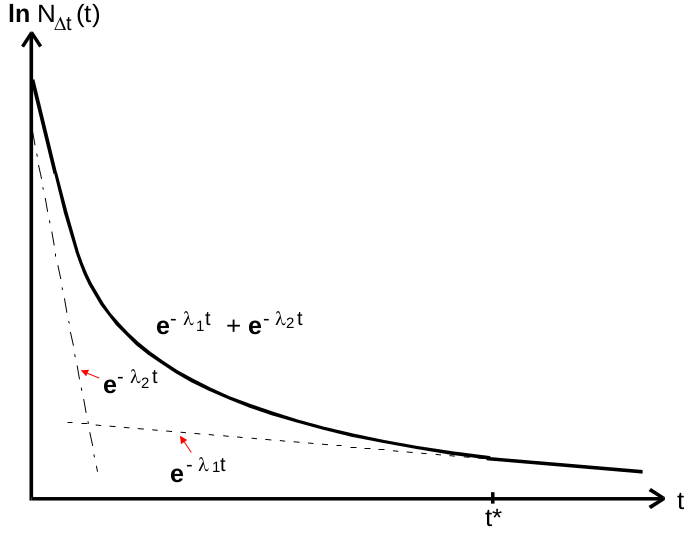
\includegraphics[scale=0.4]{silber.png}
  \caption{Zerfallsdiagramm eines Materials, dass zwei unterschiedlich langelebige Isotope besitzt \cite{anleitung}.}
  \label{fig:3}
\end{figure}

Aus \eqref{eqn:4} folgt für die Halbwertszeit
\begin{equation}
  T = \symup{ln}(2) / \lambda \, .
  \label{eqn:5}
\end{equation}
Da die Bestimmung von $N(t)$ nicht ohne weiteres möglich ist, wird eine neue Größe
$N_{\symup{\Delta t}}(t)$. Diese wird definiert als
\begin{equation}
  N_{\symup{\Delta t}}(t) = N(t) - N(t + \symup{\Delta t})
  \label{eqn:6}
\end{equation}
mit $\symup{\Delta t}$ als beliebigem Zeitintervall. Aus \eqref{eqn:4} folgt mit der Definition
\eqref{eqn:6}
\begin{equation}
  \symup{ln}[N_{\symup{\Delta t}}(t)] = \symup{ln}\left[N_0 (1 - \symup{e}^{- \lambda \symup{\Delta t}})\right] - \lambda t \, .
  \label{eqn:7}
\end{equation}
Aus \eqref{eqn:7} lässt sich mittels linearer Ausgleichsrechnung $\lambda$ und damit aus \eqref{eqn:5}
$T$ bestimmen. Das Zeitintervall $\symup{\Delta t}$ ist dabei von Material zu Material unterschiedlich
und wird angegeben.

\section{Durchführung}
\subsection{Versuchsaufbau}
Der Versuchsaufbau ist in \ref{fig:4} zu sehen. Mit dem Geiger-Müller-Zählrohr werden
die Zerfälle nachgewiesen, die Bleiummantelung soll dabei den Einfluss der Umgebungsstrahlung
minimieren. Das Gerät zum Anzeigen der Zerfälle hat dabei zwei Speicherplätze,
die laufend überschrieben werden. Das Zeitintervall, in dem gemessen werden soll,
lässt sich am Gerät einstellen.
\begin{figure}
  \centering
  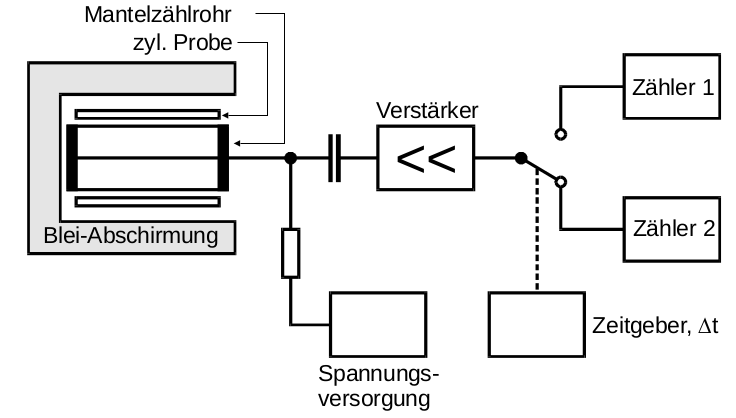
\includegraphics[scale=0.4]{aufbau.png}
  \caption{Schematischer Versuchsaufbau. \cite{anleitung}}
  \label{fig:4}
\end{figure}

\subsection{Versuchsdurchführung}
Zuerst wurde \SI{900}{\second} lang der Nulleffekt gemessen. Danach wurde zuerst für Indium 15 Messwerte
mit einem Zeitintervall $\symup{\Delta t} = \SI{4}{\minute}$ und dann für Silber 53 Messwerte mit einem
Zeitintervall $\symup{\Delta t} = \SI{8}{\second}$ bestimmt.

\section{Auswertung}
\subsection{Zur mathematischen Behandlung der Messwerte}
Die gemessenen Vorgänge unterliegen einer Poission-Verteilung, der Fehler eines
Messwertes $x_i$ ist somit durch $\sqrt{x_i}$ gegeben. Die dargestellten Ausgleichsrechnungen
wurden durch die Funktion \textsc{curve-fit} aus dem \textsc{python}-Paket \textsc{scipy.optimise}
unter berücksichtigung des Fehlers durchgeführt.
\subsection{Nullmessung}
Es wurden innerhalb von \SI{900}{\second} \num{164} Ausschläge am Geiger-Müller-Zählrohr
gemessen. Dies entspricht einem Wert von $N_\symup{null} = \SI[per-mode=reciprocal]{0.18}{\per\second}$.
Dieser Wert ist zwar gering, aber gerade bei längeren Messintervallen statistisch
signifikant, sodass er von den Messwerten abgezogen werden muss.
\subsection{Messung von Indium}
\begin{figure}
  \centering
    \begin{subfigure}{0.7\textwidth}
    \centering
      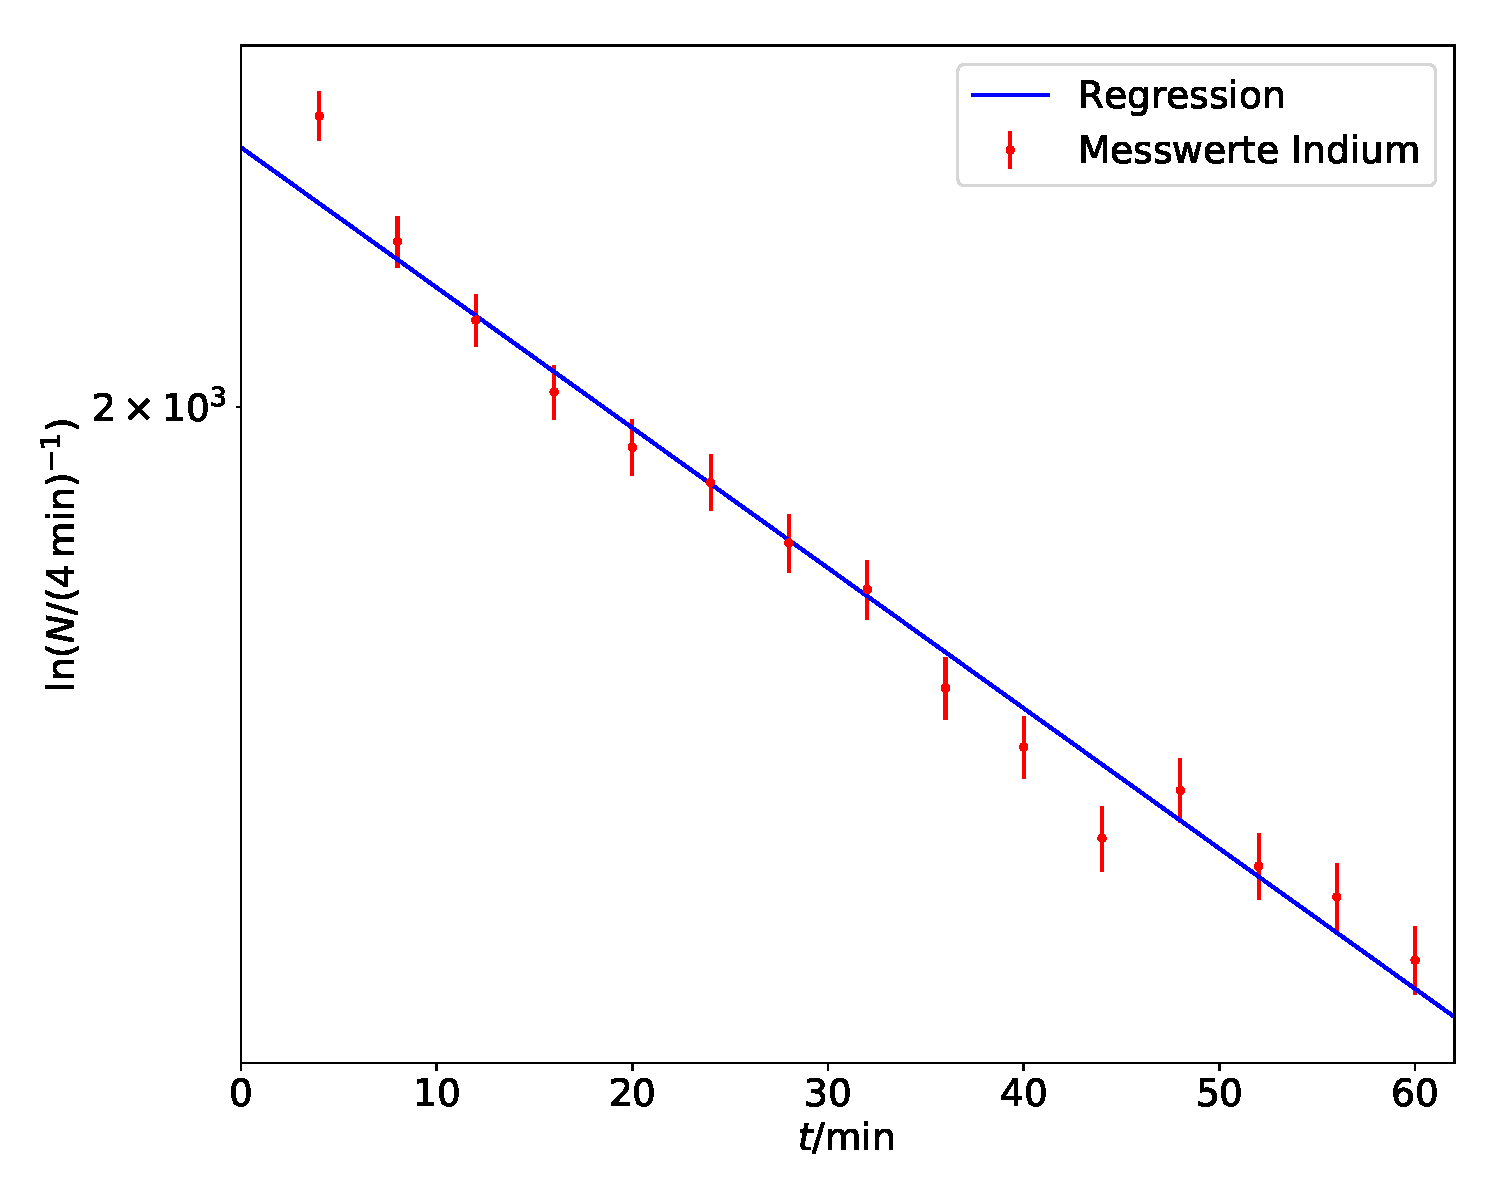
\includegraphics[width=\textwidth]{Indium.pdf}
      \caption{Grafische Darstellung der Messwerte mit Regression.}
      \label{fig:1}
    \end{subfigure}
    \begin{subtable}{0.25\textwidth}
      \centering
      \begin{tabular}{c c}
        \toprule
        t / \si{\minute} & N \\
        \midrule
        4 & 2584 \\
        8 & 2335 \\
        12 & 2192 \\
        16 & 2069 \\
        20 & 1979 \\
        24 & 1924 \\
        28 & 1833 \\
        32 & 1766 \\
        36 & 1632 \\
        40 & 1557 \\
        44 & 1448 \\
        48 & 1504 \\
        52 & 1416 \\
        56 & 1382 \\
        60 & 1314 \\
        \bottomrule
      \end{tabular}
      \caption{Messwerte.}
      \label{tab:1}
    \end{subtable}
    \caption{In Tabelle \subref{tab:1} sind die für das Isotop
    $\ce{^{116}In}$ gemessenen Werte eingetragen. Diese Werte sind
    nicht vom Nulleffekt bereinigt. In Grafik \subref{fig:1} findet sich die
    halblogarithmische Darstellung der vom Nulleffekt bereinigten Messwerte mit
    einer linearen Regression.}
  \end{figure}
  Die Messwerte finden sich in Tabelle \ref{tab:1}. Die Werte fallen mit einer
  Exponentialfunktion
  \begin{equation}
    N(t) = N_0 \symup{e}^{- \mu t}
    \label{eq:1}
  \end{equation}
  ab. Es bietet sich also eine lineare Regression mit einer Funktion
  \begin{equation*}
    n(t) = \ln{N_0} - \mu t
  \end{equation*}
  durch die logarithmierten Messwerte an. Aus \ref{eq:1} folgt weiterhin für die Halbwertszeit $T_{1/2}$:
  \begin{equation}
    T_{1/2} = \ln{\frac{1}{2}} \cdot -\mu^{-1}
    \label{eq:2}
  \end{equation}
  Es ergeben sich also folgende Konstanten:
  $N_0$:
  \begin{align*}
    \mu_\symup{In} =& \, \SI[per-mode=reciprocal]{1.91(8)e-4}{\per\second} \\
    N_{0\symup{, In}} =& \, \SI[per-mode=reciprocal]{10.3(2)}{\per\second} \\
    T_{1/2\symup{, In}} =& \, \SI{60.3(25)}{\minute}.
  \end{align*}
Die Messwerte mit Fehler sowie die berechnete Regression finden sich in Abbildung \ref{fig:1}.
\subsection{Messung von Silber}
\begin{table}
  \centering
  \begin{tabular}{c c | c c | c c | c c}
    \toprule
    t / \si{\second} & N & t / \si{\second} & N & t / \si{\second} & N & t / \si{\second} & N \\
    \midrule
    8 & 146 & 120 & 21 & \sout{232} & \sout{6} & 344 & 6 \\
    16 & 120 & 128 & 18 & \sout{240} & \sout{11} & 352 & 3 \\
    24 & 86 & \sout{136} & \sout{22} & 248 & 10 & 360 & 4 \\
    \sout{32} & \sout{87} & 144 & 16 & \sout{256} & \sout{3} & \sout{368} & \sout{15} \\
    40 & 60 & \sout{152} & \sout{22} & \sout{264} & \sout{4} & 376 & 5 \\
    \sout{48} & \sout{58} & 160 & 17 & 272 & 10 & 384 & 5\\
    56 & 43 & 168 & 15 & 280 & 9 & \sout{392} & \sout{9}\\
    \sout{64} & \sout{51} & \sout{176} & \sout{5} & \sout{288} & \sout{5} & 400 & 2 \\
    72 & 34 & 184 & 11 & 296 & 9 & 408 & 5 \\
    80 & 24 & 192 & 12 & 304 & 10 & \sout{416} & \sout{9} \\
    88 & 24 & \sout{200} & \sout{13} & \sout{312} & \sout{6} & 424 & 5 \\
    \sout{96} & \sout{26} & 208 & 9 & 320 & 10 & & \\
    104 & 23 & 216 & 9 & 328 & 10 & & \\
    112 & 24 & \sout{224} & \sout{6} & 336 & 6 & & \\
    \bottomrule
  \end{tabular}
  \caption{Messwerte der Messung an Silberisotopen.}
  \label{tab:2}
\end{table}
\begin{figure}
\centering
  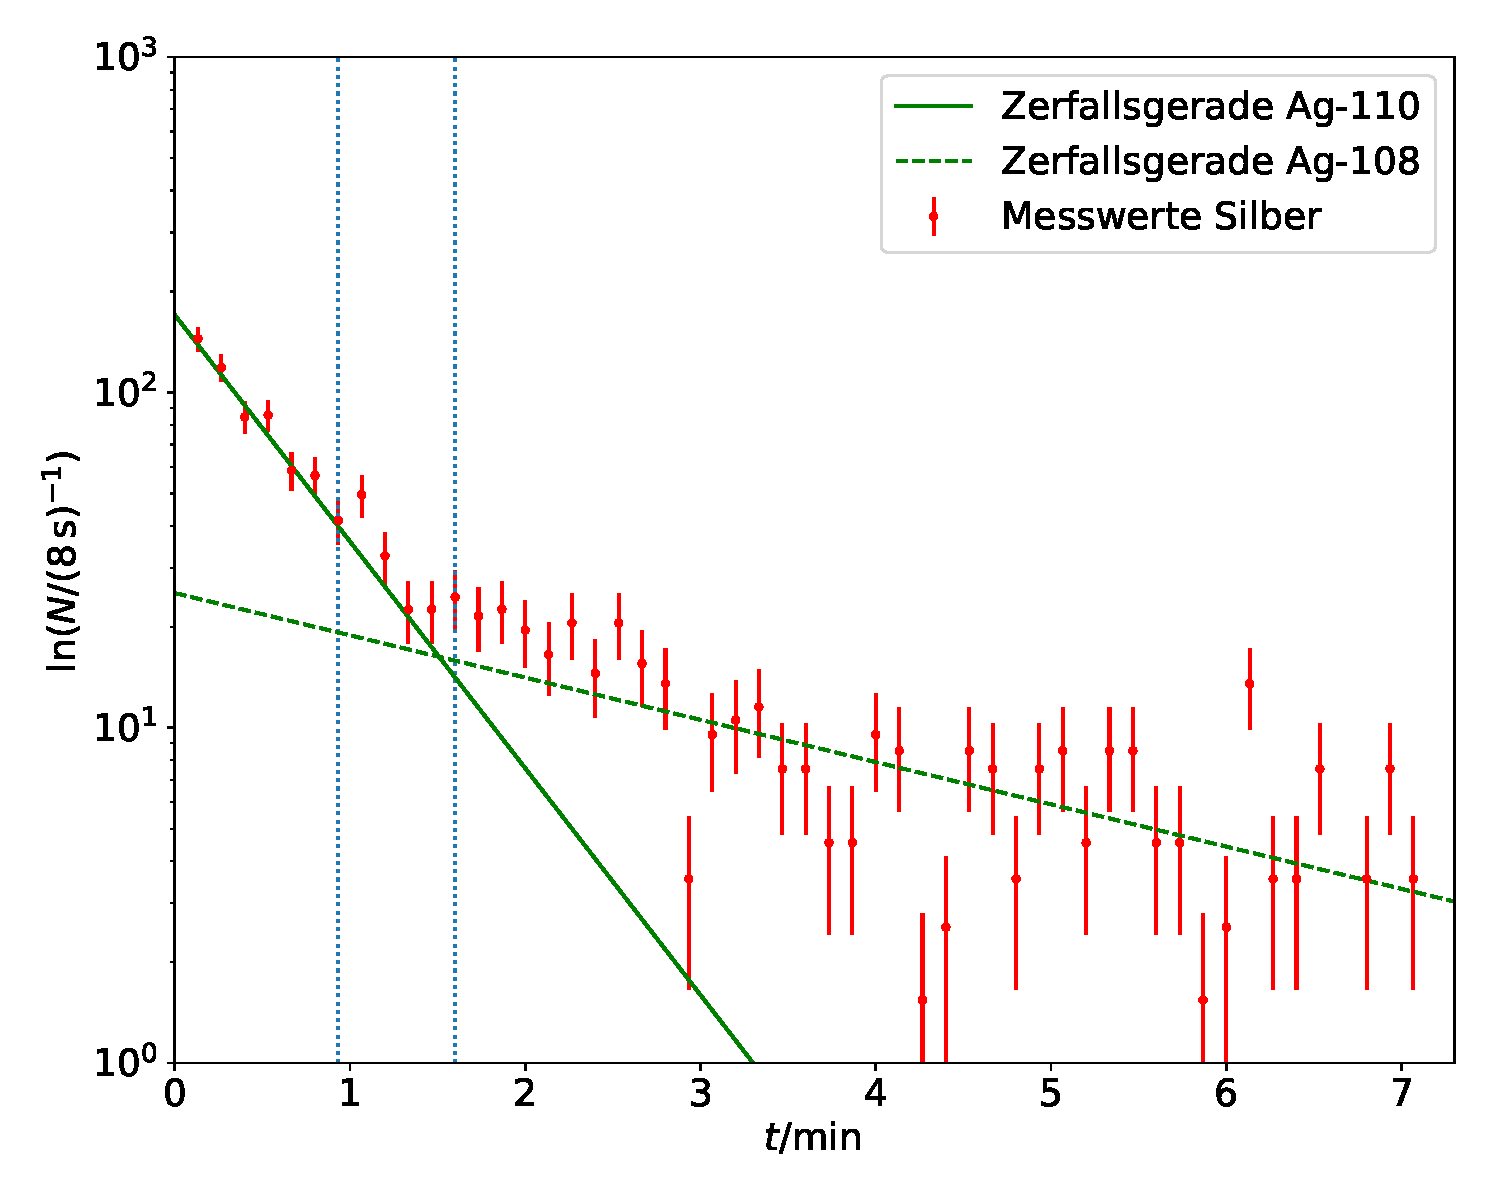
\includegraphics[width=\textwidth]{Silber.pdf}
  \caption{Diagramm der Messwerte. Die nicht betrachteten Messwerte sind ohne Angabe
  der Fehler eingetragen. Ebenfalls eingetragen sind die Zerfallsgeraden
  der Isotope $\ce{^{108}Ag}$ und $\ce{^{110}Ag}$.}
  \label{fig:2}
\end{figure}
Die Messwerte finden sich in Tabelle \ref{tab:2}. Messwerte, die deutlich als fehlerhaft
erkennbar sind, werden in den Berechnungen nicht beachtet und sind in der Tabelle
durchgestrichen. Die grafische Darstellung der Messwerte findet sich in Abbildung \ref{fig:2}
Die Messkurve lässt sich in drei Intervalle einteilen, die in der Grafik durch
gepunktete vertikale Linien getrennt sind. Im ersten Intervall dominiert das
kurzlebige $\ce{^{110}Ag}$ die gemessenen Zerfälle. In einem folgenden Übergangsintervall
kann über eine eventuelle Dominanz eines Isotops keine Aussage getroffen werden.
Im letzten Intervall überwiegt dann das langlebigere $\ce{^{108}Ag}$. Lineare
Ausgleichsrechnung durch die Messwerte der beiden relevanten Intervalle liefert
Werte für $\mu$ und $N_0$. Aus $\mu$ kann aus \eqref{eq:2} wieder die Halbwertszeit
des Isotops bestimmt werden. Für $\ce{^{110}Ag}$ ergibt sich:
\begin{align*}
  \mu_\symup{Ag-110} =& \, \SI[per-mode=reciprocal]{0.24(4)}{\per\second} \\
  N_{0\symup{, Ag-110}} =& \, \SI[per-mode=reciprocal]{17.9(16)}{\per\second} \\
  T_{1/2\symup{, Ag-110}} =& \, \SI{2.9(5)}{\second}
\end{align*}
und für $\ce{^{108}Ag}$
\begin{align*}
  \mu_\symup{Ag-108} =& \, \SI[per-mode=reciprocal]{5.6(1)e-3}{\per\second} \\
  N_{0\symup{, Ag-108}} =& \, \SI[per-mode=reciprocal]{2.4(4)}{\per\second} \\
  T_{1/2\symup{, Ag-108}} =& \, \SI{2.05(35)}{\minute}
\end{align*}
\section{Diskussion}
\begin{table}
  \centering
  \begin{tabular}{c c c c}
    \toprule
    Isotop & Quelle & $\mu$ & $T_{1/2}$\\
    \midrule
    $\ce{^{108}Ag}$ & \cite{Ag-108} & \SI[per-mode=reciprocal]{4.9e-3}{\per\second} & \SI{2.37}{\minute} \\
    $\ce{^{110}Ag}$ & \cite{Ag-110} & \SI[per-mode=reciprocal]{2.8e-2}{\per\second} & \SI{24.6}{\second} \\
    $\ce{^{116}In}$ & \cite{In-116} & \SI[per-mode=reciprocal]{2.1e-4}{\per\second} & \SI{54.29}{\minute} \\
    \bottomrule
  \end{tabular}
  \caption{Literaturwerte.}
  \label{tab:3}
\end{table}
In Tabelle \ref{tab:3} finden sich Literaturwerte für die einzellnen Isotope. Beim Vergleich
der Werte für $\ce{^{108}Ag}$ zeigen sich gute Übereinstimmungen. Der für Literaurwert für $\mu$
liegt zwar nicht im Fehlerintervall des bestimmten Wertes, die Halbwertszeit stimmt jedoch
im Bereich der Messungeauigkeit überein. Für $\ce{^{110}Ag}$ finden sich große
Abweichungen zwischen Theorie und Experiment. Die vermutliche Fehlerquelle ist die
generell kurze Halbwertszeit beider Isotope. Besonders bei $\ce{^{110}Ag}$ findet
aufgrund der geringen Halbwertszeit
auf dem Weg zwischen Anregungsbehälter und Messaufbau eine signifikante Menge an
Zerfallsprozessen statt. Das Messergebnis wird somit verfälscht. Außerdem können für
ein so kurzlebiges Isotop nur wenige Messwerte aufgenommen werden, sodass die Datenmenge
aus der die Regression bestimmt wird entsprechend klein ist. Dies ist bei dem
relativ langlebigen Isotop $\ce{^{110}Ag}$ ein geringeres Problem. Hier wird bei
langen Messdauern jedoch die Untergrundstrahlung signifikant, sodass ein Trennen
der Zerfallsprozesse vom Untergrund schwieriger wird.\\
Auch $\ce{^{116}In}$ gibt es keinen Wert, der im Bereich der Messtolleranz liegt.
Die relativen Fehler sind jedoch mit \SI{6.07}{\percent} für die Halbwertszeit
und \SI{5.24}{\percent} für die Zerfallskonstante gering. Mögliche Fehlerquelle
sind hier statistische Schwankungen. Widerholte Messungen
würde genauere Ergebnisse bringen.
\newpage
\nocite{*}
\printbibliography
